\chapter{Contribution}
\label{chap:contribution}
This chapter explains the contribution of this thesis. \Cref{sec:contributionDingNet} starts exposing all the work done to extend and evolve the DingNet simulator; \Cref{sec:contributionACOverDingNet} illustrates  the work done to support the execution of aggregate computing programs over the DingNet simulator, and in particular Protelis programs. 

\section{Extension and evolution to DingNet}
\label{sec:contributionDingNet}
This section exposes all the improvements and extensions applied to the DingNet simulator to achieve an extendible and configurable simulator, which simulates the entire LoRa-over-MQTT network. 
Previous work on the simulator were focused mainly on three areas:
\begin{enumerate}
    \item \textbf{LoRaWAN communications}: simulation of bi-directional communication between LoRa motes and LoRa gateways;
    \item \textbf{GUI}: provide a good user interface that simplifies the configuration of simulations and allows the user to see the simulations results;
    \item \textbf{Self-adaptive applications}: evaluation of algorithms to reduce the energy consumption for LoRa motes communications, but ensuring that each transmission is received at least from one gateway.
\end{enumerate}
The following part of the section discusses the contribution to the DingNet simulator (part of this work has been done in collaboration with Federico Quin, a PhD student at KU Leuven).
\clearpage
\subsection{Platform requirements}

This section illustrates the identified requirements that the platform DingNet has to satisfy to enable simulations of applications over the LoRa-over-MQTT network stack.
The requirements are grouped in functional requirements, and non-functional requirements.

\subsection*{Functional requirements}

The functional requirements are the following:
\begin{itemize}
    \item \textbf{Entities displacement and motes mobility:} the simulator has to allow to displace both the entities (gateways and motes) in the entire simulation region. It has also to allow the mote mobility in each direction to emulate realistic movement;
    \item \textbf{LoRa transmission:} the simulator has to simulate the communication between gateways and motes. This means emulate the propagation of LoRa transmissions based on the source configuration. It has to compute the transmission power decay, considering the distance from the source and the terrains crossed by the signal, in order to identify the gateways that receive the transmission. Finally, it has to be able to detect the collisions among different transmissions;
    \item \textbf{Configuration of the LoRa transmission parameters:} the platform has to support the configuration of the parameters that effect the LoRa transmissions, verifying the validity of their values. These parameters are transmission power, spreading factor, bandwidth, and code rate;
    \item \textbf{Communication protocol gateways-motes:} the MAC layer of the \mbox{LoRaWAN} protocol defines an ALOHA-like protocol to regulate the communication from mote to gateways, and three different interaction schemes to standardise the communication from gateway to mote. The simulator has to implement the simplest type of ALOHA protocol and adopt the interaction schema for the devices of ``class A" as default. However, it has to allow to change these protocols in future to evaluate the simulated systems with different ones;
    \item \textbf{Managing incoming message mote-side:} the motes entities are able to receive packets from the network-server for network administration purposes, and from the applications. So, the platform should allow to manage the incoming packets mote-side, applying actions with side effect to the mote or to the environment in accord with the packet payload;
    \item \textbf{Application layer:} it is the layer that includes the interaction between the gateways and the applications, and the involved entities. 
    This platform want to simulate LoRaWAN networks with LoRa-over-MQTT architecture, so the interactions between gateways and application are intermediated by the network-server and they are based on MQTT. 
    This layer can be composed by several services (for example the geolocation one), but the only mandatory is the network-server;
    \item \textbf{Time-frame simulations:} the platform has to allow the user to perform simulation with a predetermined duration even for more than a day. It is useful to verify how the system reacts in different scenarios and conditions that can happen in large time-frames; 
    \item \textbf{Configurable sensors:} the behaviour of the simulated applications can depend from the sensed data received from the motes. So, it is important provide configurable sensors, that guarantee to the user to define the values to produce in each zone of the simulated region in every instant.
    This is useful to simulate the applications in different scenarios, and to assure the simulation reproducibility;
    \item \textbf{Transmission statistics:} the simulator should be able to export statistics about the transmissions to evaluate and compare the different solutions simulated. Information of interest are the transmission received power from the gateways, the energy consumed by the motes, the number of collision among transmissions, the time on air of each transmission, and the transmission source position.
\end{itemize}

\subsection*{Non-functional requirements}

The identified non-functional requirement concerns with the \textbf{project maintainability}. 
In this context techniques to automatise the project life cycle have to be applied, and mainly to automatise dependency management, project build, execution of all the tests in fresh environments, enforce adoption of a common style, and optionally also deployment of the project.
Automatise all these activities is useful to increase the productivity and maintain a good quality project over time.

% build tool
% CI e CD

\subsection{Problem analysis and Design}

This section discusses the requirements above illustrated and exposes the adopted solution. 
Requirements as simulation of LoRa transmissions, configuration of their parameters, and export of transmission statistics are already satisfied, so they are not further discussed.

\subsection*{Entities displacement and motes mobility}
DingNet already allows these features, but with limitations due to the spatial reference system (SRS) of the simulation environment. The SRS is a discrete one and this leads to:
\begin{itemize}
    \item low precision in displacement of gateways and motes in the environment;
    \item mobile motes can move only in horizontal or vertical directions. 
\end{itemize}  
In order to increase the precision for the displacement of the entities and move mobile motes in each direction with straight lines, the discrete SRS is converted to a continuous one. 

\subsection*{Communication protocol gateways-motes}

Actually the simulator encapsulates the communication protocols of gateways and motes inside the class \mbox{\textit{NetworkEntity}}, that is their base class. 
This does not allow to evaluate simulated systems with different protocols, but more important this means that gateways and motes can apply only the same protocol.
The architecture proposed in \autoref{fig:sendRec} generalises the behaviour of the two entities exporting the protocol logic outside the base class with the two strategies \mbox{\textit{Sender}} and \mbox{\textit{Receiver}}. 
It grants to define different protocols for each entity allowing the motes to apply a ALOHA-like protocol, and to regulate the communication gateway-mote with the interaction schemes defined by the classes of device.
Finally, it also allows to evaluate the network behaviour with several variants of protocols.
% 
\begin{figure}[h]
    \centering
    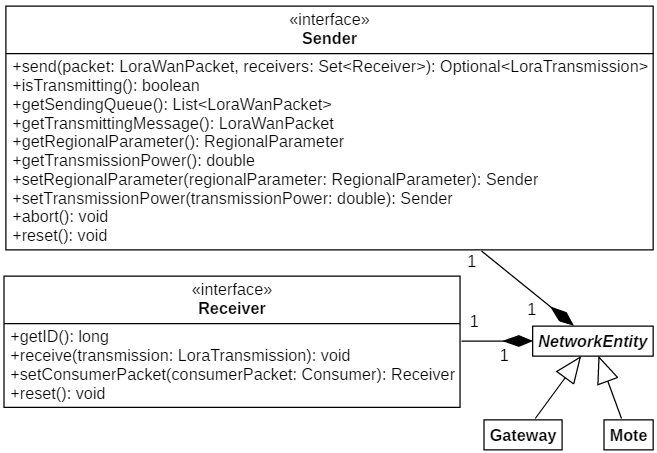
\includegraphics{figures/sendRec.png}
    \caption{\mbox{\textit{NetworkEntity}} architecture with \mbox{\textit{Sender}} and \mbox{\textit{Receiver}} interfaces.}
    \label{fig:sendRec}
\end{figure}
 
\noindent \mbox{\textit{Sender}} interface defines methods to send a packet, check the transmission status, and manage parameters that influence the transmission; while the \mbox{\textit{Receiver}} interface defines methods to receive incoming transmissions, and allows to the \mbox{\textit{NetworkEntity}} to specify how manage them.

\subsection*{Managing of incoming message mote-side}

The simulator partially supports the managing of incoming message mote-side: it is designed only the structure to manage the \textit{MAC Commands} (special commands exchange between network server and motes for network administration) motes side.
The architecture illustrated in \autoref{fig:consume} is designed to complete the managing of incoming messages to a LoRa mote, allowing to use all the information contained in the payload.
\mbox{\textit{ReceivedPacketStrategy}} defines the strategy to use to store all the incoming packets and manage the pending queue of packets to consume.
\mbox{\textit{ConsumePacketStrategy}} defines how to use the information in the payload to produce a side-effect on the LoRa mote or on the environment. 
Every mote can have a list of \mbox{\textit{ConsumePacketStrategy}}, which are performed in an ordered way with strategies that can use or ignore the packet.
\autoref{fig:consume} shows two implementations of \mbox{\textit{ReceivedPacketStrategy}}, and none of \mbox{\textit{ConsumePacketStrategy}}. This because the first strategies are cross domain while the second ones are domain specific in respect of the simulated application.
% 
\begin{figure}[H]
    \centering
    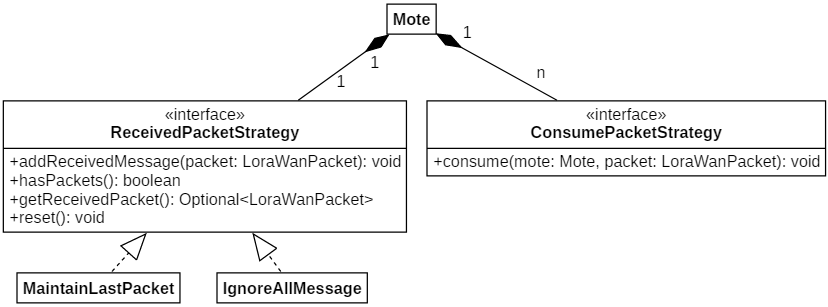
\includegraphics[width=\textwidth]{figures/consumePacket.png}
    \caption{Architecture to manage incoming packets mote side}
    \label{fig:consume}
\end{figure}
% 

\subsection*{Application layer}
The actual application layer provided by DingNet connect directly gateways and applications without the mediation of the network-server, and without use MQTT as communication technology.
So, in order to obtain the desired simulation platform, and provide realistic simulation over the LoRaWAN stack it is necessary to implements both.

\subsubsection{MQTT communication}
MQTT has to be used as communication technology for both the bi-directional communications gateways to network-server and network-server to applications, but there are no requirements that obligate to use the same broker for both the interactions. 
During the problem analysis phase the following requirements were identified for the MQTT client:
\begin{itemize}
    \item[Req1.] allow simulations with different client abstractions, optimisations, and realise a simulator technology independent for MQTT client's implementation;
    \item[Req2.] avoid MQTT messages conversions to domain specific objects at each topic \mbox{subscription}.
\end{itemize}
In order to fulfil Req1 it is necessary to allow to switch client implementation in a simple and fast way (for example from a mock implementation to a real one).
To do so the interface \mbox{\textit{MqttClient}} is defined, which allows to avoid to use directly a particular implementation.
It represents a MQTT client and it provides all the basic functionalities to interact with a MQTT broker. 
This interface grants to use custom implementations of MQTT client or external libraries implementing a wrapper extending the interface.
% 
In order to satisfy Req2 it is necessary to delegate conversions from and to the MQTT message type to the client, which interacts with the broker and knows how manipulates them.
% 
This requires to specify the receiving message type during the topic subscription phase.
% 
\autoref{fig:mqtt} shows the \mbox{\textit{MqttClient}} interface and its actual available implementations.
\begin{figure}[h]
    \centering
    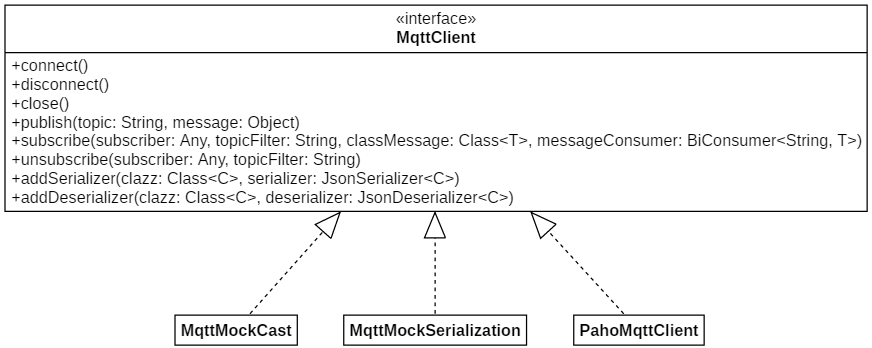
\includegraphics[width=\textwidth]{figures/mqttClient.png}
    \caption[\textit{MqttClient} interface and its available implementations]{\textit{MqttClient} interface and its available implementations. Thanks to \mbox{\textit{addSerializer}} and \mbox{\textit{addDeserializer}} methods it is possible to define custom strategies to convert messages for each client.}
    \label{fig:mqtt}
\end{figure}

\noindent The designed architecture is not valid only for this project, but it is reusable in different projects, so it is decided to export it as an external library. The library is actually available on github\footnote{\href{https://github.com/Placu95/MqttClientWrapper}{https://github.com/Placu95/MqttClientWrapper}} and a release on Maven Central Repository is planned shortly.

\subsubsection{Network server}
The network server is the entity appointed to regulate the communication between gateways and applications, but there isn't any specification that defines which tasks has to perform and which is its architecture. 
Different providers propose different solutions. 
The solution designed for the simulator is composed of an autonomous simulator entity that performs two tasks:
\begin{enumerate}
    \item filtering of duplicated messages in communication from gateways to applications;
    \item selections of the best gateway to deliver an application's message to a LoRa mote. 
    Default strategy to choose the gateway selects the gateway that has received the last transmission from the LoRa mote with more transmission power, but it is possible to change it defining different strategies. 
\end{enumerate}
\autoref{fig:GtoA} introduces the new communication schema from a gateway, which receives a LoRa transmission, to the application; while \autoref{fig:AtoG} introduces the new communication schema from an application, which wants to send a message to a LoRa mote, to the selected gateway that performs the LoRa transmission.
\begin{figure}[h]
    \centering
    \begin{subfigure}{.495\textwidth}
        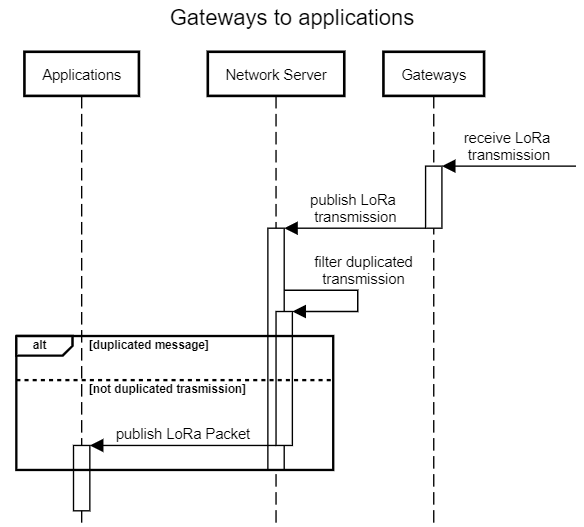
\includegraphics[scale=0.37]{figures/GtoApp.png}
        \caption{Communication from gateways \\to application}
        \label{fig:GtoA}
    \end{subfigure}
    \begin{subfigure}{.495\textwidth}
        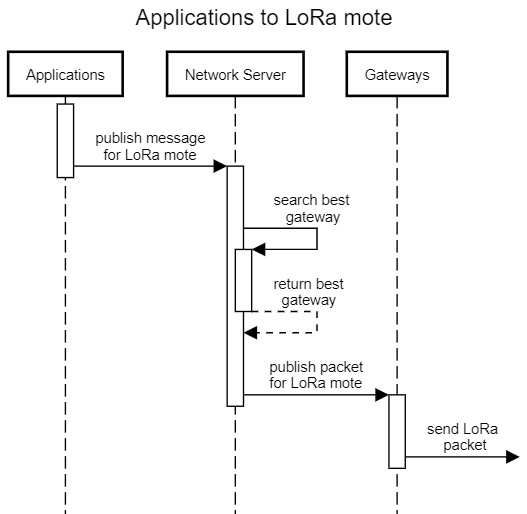
\includegraphics[scale=0.37]{figures/AppToG.png}
        \caption{Communication from application \\to gateways}
        \label{fig:AtoG}
    \end{subfigure}
    \caption{Communications between gateways and applications}
    \label{fig:netSer}
\end{figure}

\subsection*{Time-frame simulations}
The platform actually does not support time-frame simulations, but only single run simulations, and multiple run simulations.
A single run simulation finishes when all the mobile LoRa motes arrive at the respective destination, while a multi run consists simply in run more time a single run simulation.
So, it is necessary to define a new type of simulation that satisfy the requirement.
Another problem is the impossibility to perform simulation of more than a day dues to the actual time representation.
\textit{Timed run} is the new type of simulation introduced to go beyond the limitations of the single run one. 
This type of simulation differs from the single run only for the termination condition. 
The condition requires to define the duration of the simulation, so the condition evaluates it as finished when the defined time is passed.
In order to enable simulation of more than a day, 
%   
\begin{figure}[!b]
    \centering
    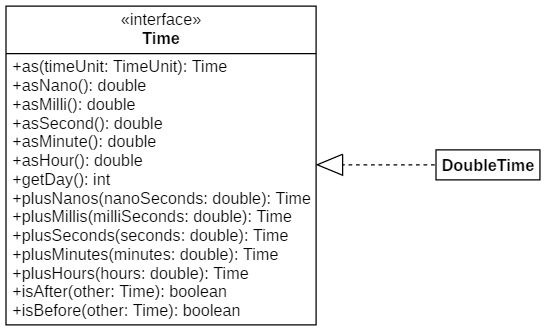
\includegraphics{figures/time.png}
    \caption[Time representation in DingNet simulator]{Time representation that provides all the basic functionalities.}
    \label{fig:time}
\end{figure}
% 
it is necessary to change the time representation from the java class \mbox{\textit{LocalTime}} to a new one.
The new time representation is proposed in \autoref{fig:time}.
It does not enable only multi-days simulation, but also it simplifies the time manipulation providing methods for the different unit of measure, including the milliseconds that are the default one used by the simulator.


\subsection*{Configurable sensors}
DingNet already defines its own concept of sensor defined by the interface \mbox{\textit{SensorDataGenerator}}, and some its implementations.
The problem is that miss a support to configure with low effort the values that the sensors has to produce.
In order to solve the problem, it wants to define an extendible architecture starting from the sensor interface already defined, which grants to configure the values to produce.
The idea is to have sensors that produce values in a configurable way splitting the region of simulation in a matrix of configurable dimension.
So for each cell of the matrix it is defined a list of configurations. 
Each cell's configuration defines the starting time of validity and the range of producible values. 
Then starting from this configuration is produced a tricubic spline interpolation function where the three variable are: the two coordinates of the matrix and the time; while the result is the corresponding sensor value.
Finally, when a mote requires a new value to the sensor, it produces the value considering the mote position and the simulation time.
The result is that each sensor inside the same cell produces the same value at the same time. 
The architecture of this sensor is showed in \autoref{fig:rangedSensor}, and:
\begin{itemize}
    \item \textbf{Cell} represent the cells that compose the configurable matrix;
    \item \textbf{RangeValue} is the range of validity for the value to produce;
    \item \textbf{RangeDataGenerator} is the abstract class that loads the configuration file of the sensor, generates the interpolating function and produces values for LoRa motes. It requires only to define the type of the two interfaces \textit{Cell} and \textit{RangeValue}.
\end{itemize}
% 
\begin{figure}[h]
    \centering
    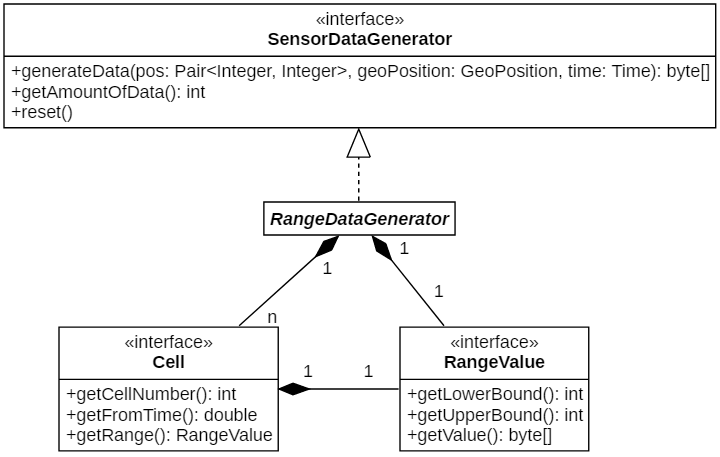
\includegraphics[scale=0.8]{figures/rangedSensor.png}
    \caption{Architecture of the configurable sensor}
    \label{fig:rangedSensor}
\end{figure}
% 
In order to define new configurable sensors it is require only to implement the \mbox{\textit{RangeDataGenerator}} abstract class specifying the type of \mbox{\textit{Cell}} and \mbox{\textit{RangeValue}}.
The actual file format for the sensor configuration file is \textit{toml}\footnote{\href{https://github.com/toml-lang/toml}{https://github.com/toml-lang/toml (Feb 2020)}}, but thanks to the \textit{konf}\footnote{\href{https://github.com/uchuhimo/konf}{https://github.com/uchuhimo/konf (Feb 2020)}} library (used to parse the file) it will be possible to change the file format with low effort.

\subsection*{Project maintainability}
In order to automatise the dependency management, and the project build was evaluated two build tool: \textit{Apache Maven} and \textit{Gradle}.
\textit{Gradle} is preferred to \textit{Apache Maven} for several reasons\footnote{\href{https://gradle.org/maven-vs-gradle/}{https://gradle.org/maven-vs-gradle (Feb 2020)}}. The main ones are: performance, highest readability of the project's configuration file due to a less verbose syntax, and better script support (with the possibility to write them in kotlin with \textit{Gradle Kotlin DSL}).
Instead, \textit{Travis-CI}\footnote{\href{https://travis-ci.com/}{https://travis-ci.com (Feb 2020)}} is chosen as continuous integration service to run a new build of the project and execute all its test in fresh environments after every change.
Travis-CI is chosen because it is free, well integrated with \textit{GitHub} which hosts the project, and support to automatise the deployment.
It is configured to test the project in all the main operative systems (linux, windows, and osx) and with different java versions (11 and 12), but is not configured to automatise the deployment.
Finally, \textit{Checkstyle}\footnote{\href{https://checkstyle.sourceforge.io/}{https://checkstyle.sourceforge.io/ (Feb 2020)}} is adopted to enforce the use of a common style in the entire project, and its execution is planned every time Travis-CI performs all the class of tests. 

\clearpage
\section{Aggregate programming over a LoRa-over-MQTT network}
\label{sec:contributionACOverDingNet}
This section discusses the integration between the aggregate computing paradigm and a LoRa-over-MQTT network like DingNet; enabling the simulation of aggregate applications on this platform.
In order to join these two concepts, at first is necessary to define how to map the networks entities in an aggregate computing system, and second identifies potentially additional requirements or limitations for these entities.
In the aggregate computing viewpoint, a system is composed of a set of distributed heterogeneous computational entities, called nodes. Nodes execute the same global program and communicate with a subset of them defined by a neighbourhood policy. 
While, in a LoRaWAN network the main entities are: LoRa motes, gateways, and network server; but at application level the only interesting entities are the LoRa motes.
So, following the aggregate vision it is natural to map each LoRa mote in a node that represents its digital twin (from now on called LoRa node) inside the aggregate system.
\\On the one hand, LoRa nodes can be considered as generic nodes and they do not require any specific neighbourhood's policy, or the use of particular communication technology to interact with their neighbours. 
But on the other hand, they have to support communication via MQTT to enable bidirectional communication with the respective physical counterparts.
Finally, it is necessary to analyse if all the network entities, or only some of them, can host the aggregate nodes.
In \cite{CCNCPS2018} the authors propose a software architecture to enable the execution of aggregate computing programs on LoRa motes, but after evaluations of the proposed solution, they identify some issues due to the physical limitations of the communication technology. 
These issues do not allow to execute aggregate computing program directly on the LoRa motes, but they are not valid for the other network entities and there is any paper that identifies others possible issues.
Even if all the LoRaWAN network entities excluded the motes can host the aggregate node (LoRa nodes or other types of nodes), it is important to specify a limitation for the LoRa nodes. 
The LoRa nodes can interact with the respective LoRa mote only following the interaction schema defined from the LoRa-over-MQTT networks. 
For example, if a LoRa node is hosted by a LoRa gateway, that receives directly the transmissions of the respective LoRa mote, it cannot receive directly the packet, but it has to wait that the packet is published on the MQTT broker.

\subsection{Integration of Protelis with DingNet}
\label{sec:PoverD}
% The following subsection presents the software architecture designed to support the LoRa nodes inside an aggregate computing system defined in \textit{Protelis}.
The only things to do to enable the development of Protelis applications over the DingNet network is to satisfy the requirement previously identified.
That requirement represents a specific capability of this type of nodes and Protelis defines a single place appointed to host it, the \mbox{\textit{ExecutionContext}}.
\autoref{fig:execContext} shows the model of the \mbox{\textit{ExecutionContext}} designed for the LoRa nodes. 

\begin{figure}[h]
    \centering
    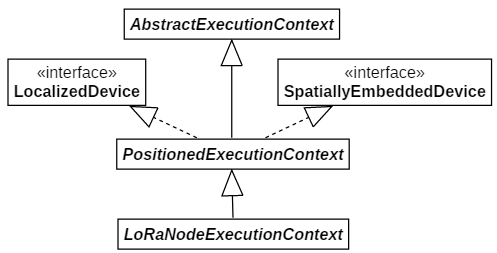
\includegraphics{figures/execContext.png}
    \caption{Model of \textit{ExecutionContext} for LoRa nodes}
    \label{fig:execContext}
\end{figure}

\noindent For devices spatially embedded and mainly used to transmit sensor values, their position is a relevant information. So, \mbox{\textit{PositionedExecutionContext}} is defined, which extends \mbox{\textit{AbstractExecutionContext}} (provided by Protelis) implementing the two interfaces that define functions to obtain spatial information of the device.
\mbox{\textit{LoRaNodeExecutionContext}} is the basic execution context for a LoRa node that:
% 
\begin{itemize}
    \item adds support for MQTT communication, satisfying the identified requirement;
    \item encapsulates the subscription to the MQTT topic to receive the sensed values from the respective LoRa mote;
    \item manages the received packet adding the sensed values to the knowledge-based of the node, or modifying its position if the value belongs to the GPS sensor.
\end{itemize}
% 
The introduced model enables the design of Protelis application composed of LoRa nodes, but also of not LoRa nodes.
Protelis applications with the model illustrated in \autoref{fig:appP} are not only valid for the DingNet network but for all the LoRa-over-MQTT networks that provide LoRa mote's data on a MQTT broker.
% 
\begin{figure}[h]
    \centering
    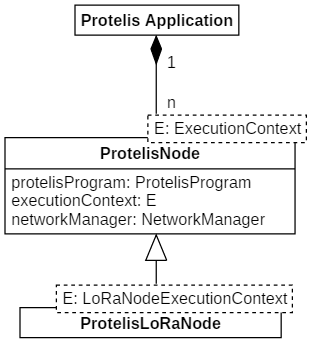
\includegraphics{figures/app.png}
    \caption{Abstract model of a Protelis application composed of LoRa nodes}
    \label{fig:appP}
\end{figure}
% 
\noindent In order to execute Protelis applications on the top of DingNet simulator, enabling the simulation of Protelis applications composed of LoRa nodes, one last small operation is necessary: unify the concept of time. 
This operation is necessary because the behaviour of every Protelis node depends also from the time in which their execution is scheduled, and the LoRa packets are received.
To do this it is sufficient wrapping the \mbox{\textit{LoRaNodeExecutionContext}} using the simulator time concept.

\paragraph{Concluding remarks.} This chapter discussed the main works done during this thesis. First it exposed the main improvements and evolution on DingNet simulator. Then it illustrated the support to simulate Protelis application inside the DingNet simulator.